\documentclass[9pt,twocolumn,twoside]{../../styles/osajnl}
\usepackage{fancyvrb}
\usepackage{graphicx}
\journal{i524} 


\title{An overview of Apache THRIFT and its architecture}

\author[1]{Karthik Anbazhagan}

\affil[1]{School of Informatics and Computing, Bloomington, IN 47408, U.S.A.}

\affil[*]{Corresponding authors: kartanba@iu.edu}

\dates{\today}

\ociscodes{Cloud, Apache Thrift, cross-language, I524}

% replace this with your url in github/gitlab
\doi{\url{https://github.com/cloudmesh/sp17-i524/tree/master/paper2/S17-IR-2008/report.pdf}}



\begin{abstract}
Thrift \cite{wiki-thrift} is a software framework developed at Facebook to expedite the development and implementation of efficient and scalable cross-language development services \cite{thrift-paper-2013}. Its primary goal is to enable efficient and reliable communication across programming languages by abstracting the portions of each language that tend to require the most customization into a common library that is implemented in each language. This paper speculates the feasibility of using a such a system and looks deeper into the different ways you can use it and show how Apache Thrift can fulfill any needs with the flexibility it provides in choosing the different layers of the architecture separately.
\end{abstract}
\setboolean{displaycopyright}{true}

\begin{document}

\maketitle
\tableofcontents % Print the contents section
\section{Introduction}
Apache Thrift is an Interface Definition Language \cite{www-thrift-idl} (IDL) used to define and create services between numerous languages as a Remote Procedure Call (RPC). Its lightweight framework and support for cross-language communication makes it more robust and efficient compared to other RPC frameworks like SOA \cite{blog-thrift} (REST/SOAP). It allows you to create services that are usable by numerous languages through a simple and straightforward IDL. It combines a software stack with a code generation engine to build services that works efficiently and seamlessly between $C++$, Java, Python, PHP, Ruby, Erlang, Perl, Haskell, C, Cocoa, JavaScript, Node.js, Smalltalk, and OCaml. In addition to interoperability, Thrift can be very efficient because of a serialization mechanism \cite{git-thrift-serial} which can save both space and time. In other words, Apache Thrift lets you create a service to send/receive data between two or more softwares that are written in completely different languages/platforms. \\

Thrift was originally developed at Facebook and is one of the “core parts of their infrastructure”. The choice of programming language at Facebook was based on what language was best suited for the task at hand. This flexibility resulted in difficulties when these applications needed to call one another and Facebook needed an application that could meet their needs of interoperability, transport efficiency, and simplicity. Out of this need, they developed efficient protocols and a service infrastructure which became Thrift. Facebook decided to make Thrift an Open Source and finally contributed it to Apache Software Foundation (ASF) in April 2007 in order to increase usage and development. Thrift was later released under the Apache 2.0 license.

\section{Architecture}

Figure. 1 shows the architecture of a model for using the Thrift Stack. It is very essential to understand every component of the architecture to understand how Apache Thrift works. This section describes in brief about the components that are part of the Thrift architecture. It includes a complete stack for creating clients and servers. The top portion of the stack is the user generated code from the Thrift Client-Server definition file. The next layer of the framework are the Thrift generate client and processor codes which also comprises of data structures. The next two important layers are the protocol and transport layers which are part of the Thrift run-time libraries. This provides Thrift the freedom to define a service and change the protocol and transport without regenerating any code. Thrift includes a server infrastructure to tie the protocols and transports together. There are blocking, non-blocking, single and multi-threaded servers. The 'Physical' portion of the stack varies from stack to stack based on the language. For example, for Java and Python network I/O, the built-in libraries are leveraged by the Thrift library, while the C++ implementation uses its own custom implementation. Thrift allows users to choose independently between protocol, transport and server. With Thrift being originally developed in C++, Thrift has the greatest variation among these in the C++ implementation \cite{www-thrift-example}.

\begin{figure}[h]
    \centering
    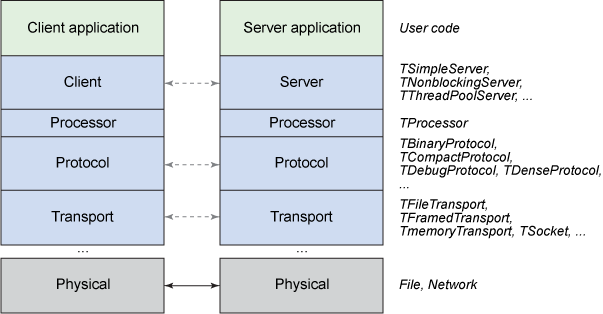
\includegraphics[width=3.5in]{images/thrift_arch.png}
    \caption{Architecture of Apache Thrift  \cite{www-thrift-arch}}
    \label{fig:thrift_arch}
\end{figure}


\subsection{Transport Layer}
The transport layer provides simple abstraction for read/write to/from the network. Each language must have a common interface to transport bidirectional raw data. The transport layer describes how the data is transmitted. This layer seperates the underlying transport from the rest of the system, exposing only the following interface:
\begin{enumerate}
	\item open: Opens the tranpsort
	\item close: Closes the tranport
	\item isOpen: Indicates whether the transport is open
	\item read: Reads from the transport
	\item write: Writes to the transport
	\item flush: Forces any pending writes\\
\end{enumerate}
There are multiple transports supported by Thrift:
\begin{enumerate}
	\item \textbf{TSocket}: The TSocket class is implemented across all target languages. It provides a common, simple interface to a TCP/IP stream socket and uses blocking socket I/O for transport.
	\item \textbf{TFramedTransport}: The TFramedTransport class transmits data with frame size headers for chunking optimization or non-blocking operation
	\item \textbf{TFileTransport}: The TFileTransport is an abstraction of an on-disk file to a data stream. It can be used to write out a set of incoming Thrift requests to a file on disk
	\item \textbf{TMemoryTransport}: Uses memory for I/O operations. For example, The Java implementation uses a simple ByteArrayOutput stream
	\item \textbf{TZlibTransport}: Performs compression using zlib. It should be used in conjunction with another transport
\end{enumerate}

\subsection{Protocol Layer}
The second major abstraction in Thrift is the separation of data structure from transport representation. While transporting the data, Thrift enforces a certain messaging structure. That is, it does not matter what method the data encoding is in, as long as the data supports a fixed set of operations that allows it to be read and written by generated code. The Thrift Protocol interface is very straightforward, it supports two things: bidirectional sequenced messaging, and encoding of base types, containers, and structs.

Thrift supports both text and binary protocols. The binary protocols almost always outperforms text protocols, but sometimes text protocols may prove to be useful in cases of debugging. The Protocols available for the majority of the Thrift-supported languages are:
\begin{enumerate}
	\item \textbf{TBinaryProtocol}: A straightforward binary format encoding takes numeric values as binary, rather than converting to text
	\item \textbf{TCompactProtocol}: Very efficient and dense encoding of data. This protocol writes numeric tags for each piece of data. The recipient is expected to properly match these tags with the data
	\item \textbf{TDenseProtocol}: It’s similar to TCompactProtocol but strips off the meta information from what is transmitted and adds it back at the receiver side
	\item \textbf{TJSONProtocol}: Uses JSON for data encoding
	\item \textbf{TSimpleJSONProtocol}: A write-only protocol using JSON. Suitable for parsing by scripting languages.
	\item \textbf{TDebugProtocol}: Sends data in the form of human-readable text format. It can be well used in debugging applications involving Thrift.
\end{enumerate}


\subsection{Processor Layer}
A processor encapsulates the ability to read data from input streams and write to output streams. The processor layer is the simplest layer. The input and output streams are represented by protocol objects. Service-specific processor implementations are generated by the Thrift compiler and these generated codes make the Process Layer of the architecture stack. The processor essentially reads data from the wire (using the input protocol), delegates processing to the handler (implemented by the user), and writes the response over the wire (using the output protocol).

	
\subsection{Server Layer}	
A server pulls together all the various functionalities to complete the Thrift server layer. First, it creates a transport, then specifies input/output protocols for the transport. It then creates a processor based on the I/O protocols and waits for incoming connections. When a connection is made, it hands them off to the processor to handle the processing. Thrift provides a number of servers:
\begin{enumerate}
	\item \textbf{TSimpleServer}: A single-threaded server using standard blocking I/O socket. Mainly used for testing purposes
	\item \textbf{TThreadPoolServer}: A multi-threaded server with N worker threads using standard blocking I/O. It generally creates five minimum threads in the pool if not specified otherwise
	\item \textbf{TNonBlockingServer}: A multi-threaded server using non-blocking I/O
	\item \textbf{THttpServer}: A HTTP server (for JS clients)
	\item \textbf{TForkingServer}: Forks a process for each request to server\\
\end{enumerate}


\section{Advantages of Thrift}
A few reasons where Thrift is robust and efficient compared to other RPC frameworks are:
\begin{itemize}
\item Thrift leverages the cross-language serialization with lower overhead than alternatives such as SOAP due to use of binary format
\item Thrift generates the client and server code completely \cite{www-thrift-tutorial}, including the data structures passed by the user, leaving the user with the only task of writing the handlers and invoking the client. Everything including the parameters and returns are automatically validated and parsed
\item Thrift is more compact than HTTP and can easily be extended to support things like encryption, compression, non blocking IO, etc
\item Thrift supports persistent connections and avoids the continuous TCP and HTTP handshakes that HTTP incurs
\item Because Protocol Buffers \cite{www-protocol-buffers} are implemented in a variety of languages, they make interoperability between polyglot applications simpler\\
\end{itemize}

\section{Limitations of Thrift}
A few reasons where Thrift is limited compared to other RPC frameworks are:
\begin{itemize}
\item Thrift \cite{pdf-thrift-tutorial} is limited to only one service per server
\item There can be no cyclic structs. Structs can only contain structs that have been declared before it. A struct also cannot contain itself
\item Important OOP concepts like inheritance and polymorphism are not supported
\item Null cannot be returned by a server. Instead a wrapper struct or value is expected
\item No out-of-the-box authentication service available between server and client
\item No Bi-Directional messaging is available\\
\end{itemize}


\section{Conclusion}
This paper has given an overview of Thrift \cite{pdf-thrift-tutorial} and its architecture and the different ways you can use it. Apache Thrift can fulfill any needs with the flexibility it provides in choosing the different layers of the architecture separately. It outmatches any other similar technology available by providing more language support and flexibility. Thrift has enabled Facebook to build scalable back-end services efficiently. It has been employed in a wide variety of applications at Facebook, including search, logging, mobile, ads, and the developer platform. Application developers can focus on application code without worrying about the sockets layer.

\bibliography{references}

\end{document}
